%%%%%%%%%%%%%%%%%%%%%%%%%%%%%%%%%%%%%%%%%%%%%%%%%%
\begin{frame}{Überblick über die Präsentation}

\Large{Specification by Example}

\vspace{2em}

\begin{itemize}

	\item Motivation
	\begin{itemize}
		\item Wen geht es an?
		\item Welche Probleme werden adressiert?
	\end{itemize}


	\item Ziel
	\begin{itemize}
		\item Was erhalten wir, wenn wir das richtig anwenden?
	\end{itemize}

	\item Weg
	\begin{itemize}
		\item Wie kommen wir dahin?
	\end{itemize}

	\item Beispiel
	\begin{itemize}
		\item Wie kann so etwas aussehen?
	\end{itemize}
\end{itemize}

\end{frame}


%%%%%%%%%%%%%%%%%%%%%%%%%%%%%%%%%%%%%%%%%%%%%%%%%%
\begin{frame}{Software aus verschiedenen Perspektiven}

\begin{itemize}

	
	\item Auftraggeber:

	\begin{itemize}
		\item \glqq Die Software soll tun, was ich erwarte.\grqq
		\item \glqq Ich will das Ganze möglichst preiswert.\grqq
	\end{itemize}
	
	
	\item Entwickler:
	
	\begin{itemize}
		\item \glqq Ich will wissen, was ich entwickeln soll.\grqq
		\item \glqq Wann bin ich fertig?\grqq
	\end{itemize}
	
	
	\item Nach der Lieferung:
	
	\begin{itemize}
		\item \glqq Was macht die Software genau?\grqq
		\item \glqq Bug oder Feature?\grqq
	\end{itemize}
\end{itemize}

\end{frame}


%%%%%%%%%%%%%%%%%%%%%%%%%%%%%%%%%%%%%%%%%%%%%%%%%%
\begin{frame}{Die Vision -- Eine Quelle für alle}

\begin{itemize}
	\item Beschreibung der Anforderung
	\begin{itemize}
		\item Alle sollen das gleiche Verständnis haben
	\end{itemize}

	
	\item Akzeptanztests für die Entwicklung
	\begin{itemize}
		\item Überprüfbare Kriterien
		\item Werden im Laufe der Entwicklung \glqq begrünt\grqq
	\end{itemize}

	
	\item Ausführbare Dokumentation
	\begin{itemize}
		\item Die Dokumentation muss zur Anwendung passen
		\item Hilfestellung bei Supportfällen
	\end{itemize}
\end{itemize}

\vspace{1em}

$\Rightarrow$ Single Source of Truth

\end{frame}


%%%%%%%%%%%%%%%%%%%%%%%%%%%%%%%%%%%%%%%%%%%%%%%%%%
%\begin{frame}{Was wir dazu brauchen}
%
%\begin{itemize}
%	\item Ein einziges Repository für die Informationen
%	\item Mit Beschreibung \em und \em Beispielen
%	\item Für jeden lesbar und verständlich formuliert
%        \item Beispiele als Akzeptanztests ausführbar
%
%	\item Gängige Tools:
%	\begin{itemize}
%		\item BDD-Tools wie Cucumber (http://cukes.info)
%		\item Webbasiert wie Concordion (http://www.concordion.org)
%		\item Tabellenbasiert wie Fitnesse (http://www.fitnesse.org)
%	\end{itemize}
%\end{itemize}
%
%\end{frame}



%%%%%%%%%%%%%%%%%%%%%%%%%%%%%%%%%%%%%%%%%%%%%%%%%%%
%\begin{frame}{Cucumber}
%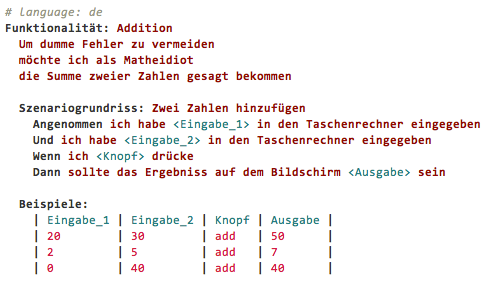
\includegraphics[width=\textwidth]{Cucumber.png} \newline
%\end{frame}
%
%
%%%%%%%%%%%%%%%%%%%%%%%%%%%%%%%%%%%%%%%%%%%%%%%%%%%
%\begin{frame}{Concordion}
%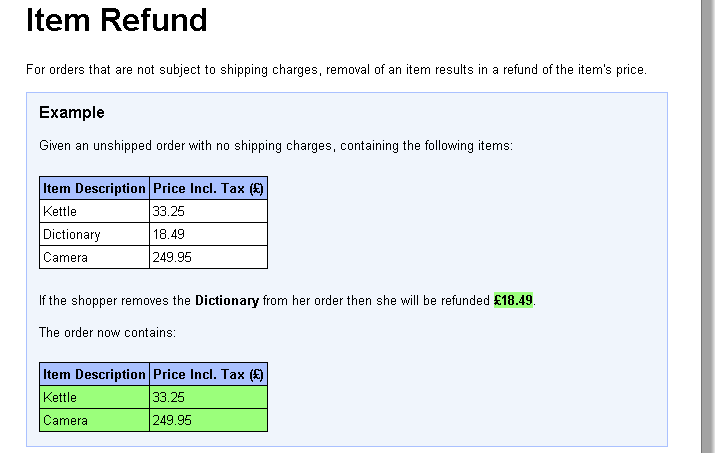
\includegraphics[width=\textwidth]{Concordion.png} \newline
%\end{frame}
%
%
%%%%%%%%%%%%%%%%%%%%%%%%%%%%%%%%%%%%%%%%%%%%%%%%%%%
%\begin{frame}{Fitnesse}
%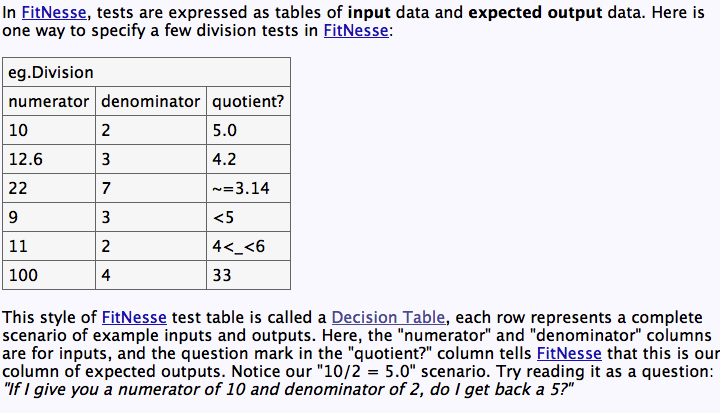
\includegraphics[width=\textwidth]{Fitnesse.png} \newline
%\end{frame}

%%%%%%%%%%%%%%%%%%%%%%%%%%%%%%%%%%%%%%%%%%%%%%%%%%
\begin{frame}{Wie wir dahin kommen}


\begin{itemize}
	\item Kommunikation und Diskussion \em aller \em Beteiligten 
	\begin{itemize}
		\item Unterschiedliche Sichtweisen und Erfahrungen
		\item Schneller Informationsfluss durch Fragen und direkte Antworten
		\item Entdecken von Widersprüchen, Lücken, Missverständnissen
		\item Stille Annahmen werden explizit
		\item Gemeinsames Verständnis entsteht
	\end{itemize}
	
	\item Fokus
	\begin{itemize}
		\item Konzentration auf die fachlich wichtigen Aspekte
                \item Strukturiertes Vorgehen
		\item Ziel: Schaffung der Single Source of Truth
	\end{itemize}
\end{itemize}


\vspace{1em}

$\Rightarrow$ Specification Workshops

\end{frame}


%%%%%%%%%%%%%%%%%%%%%%%%%%%%%%%%%%%%%%%%%%%%%%%%%%
%\begin{frame}{Specification Workshop}
%
%\begin{itemize}
%	\item Teilnehmer: 
%	\begin{itemize}
%		\item Auftraggeber, Kunde, Product Owner
%		\item Entwickler
%		\item Tester, QA-Personen
%	\end{itemize}
%	\item Zeit: 
%	\begin{itemize}
%		\item Unbedingtes Timeboxing
%		\item ca. 4 Stunden für 2 Wochen Entwicklung
%	\end{itemize}
%	\item Moderator zur Sicherstellung von: 
%	\begin{itemize}
%		\item Fokussierung
%		\item Ergebniserreichung
%	\end{itemize}
%\end{itemize}
%
%\end{frame}



%%%%%%%%%%%%%%%%%%%%%%%%%%%%%%%%%%%%%%%%%%%%%%%%%%
\begin{frame}{So kann ein Specification Workshop ablaufen}

\begin{itemize}
	\item Der Auftraggeber beschreibt sein zu lösendes Problem
	\item Die anderen Teilnehmer befragen ihn, um Klarheit zu erhalten
	\item Alle erarbeiten gemeinsam Beispiele
	\item Die Beispiele werden zusammengeführt und auf das Wesentliche reduziert
	\item Aus den Beispielen wird die ihnen zugrundeliegende Spezifikation abgeleitet
\end{itemize}

\end{frame}


%%%%%%%%%%%%%%%%%%%%%%%%%%%%%%%%%%%%%%%%%%%%%%%%%%
%\begin{frame}{Was ein Specification Workshop \em nicht \em ist}
%
%Der Workshop ist...
%
%\begin{itemize}
%	\item ... kein Meeting
%	\begin{itemize}
%		\item \emph{Ergebnisse} erzielen
%	\end{itemize}
%	
%	\item ... keine Präsentation
%	\begin{itemize}
%		\item Die Ergebnisse \emph{miteinander} erarbeiten
%	\end{itemize}
%	
%	\item ... keine technische Design Session
%	\begin{itemize}
%		\item \emph{Fachliche} Klarheit herstellen
%	\end{itemize}
%	
%\end{itemize}
%
%\onslide+<2->
%	
%$\Rightarrow$ Es ist Aufgabe des Moderators, dies sicherzustellen
%
%\end{frame}


%%%%%%%%%%%%%%%%%%%%%%%%%%%%%%%%%%%%%%%%%%%%%%%%%%
\begin{frame}{Darauf sollte man achten}

\begin{itemize}
	\item Komplizierte Beispiele
	\begin{itemize}
		\item Wo liegt die Ursache der Kompliziertheit?
		\item Es geht vermutlich einfacher
		\item Oft hilft ein Aufteilen nach Aspekten
	\end{itemize}
	
	
	\item Namensgebung
	\begin{itemize}
		\item Alle wesentlichen Konzepte brauchen klare, \emph{fachlich} verständliche Namen
		\item Jeder soll unter einem Begriff dasselbe verstehen
		\item Ein verwendeter Begriff muss in der gesamten Anwendung (und im Code!) dieselbe Bedeutung haben
	\end{itemize}
	
	
	\item Formeln
	\begin{itemize}
		\item Verschleiern oft wichtige Details oder implizite Annahmen
		\item Müssen hinterfragt und verstanden werden
	\end{itemize}
	
	
	\item Bei vielen Teilnehmern: Erstellung der Beispiele in Kleingruppen
\end{itemize}

\end{frame}



%%%%%%%%%%%%%%%%%%%%%%%%%%%%%%%%%%%%%%%%%%%%%%%%%%
\begin{frame}{Von den Beispielen hin zur Spezifikation}

\begin{itemize}
	\item Aus den Beispielen wird die Spezifikation abgeleitet und gegen die Eingangsfragen geprüft
	\item Dadurch kann man die Vollständigkeit in beide Richtungen prüfen
	\item Muss auch von jemand verstanden werden, der nicht am Workshop teilgenommen hat
	\item Die Spezifikation fasst die Beispiele zusammen
\end{itemize}

\end{frame}
 
%%%%%%%%%%%%%%%%%%%%%%%%%%%%%%%%%%%%%%%%%%%%%%%%%%
\begin{frame}{Beispiel: Konkrete Anforderung}

\begin{itemize}
	\item Ich bin Inhaber eines Hot Dog Standes und habe schon ein kleines Kassensystem mit Bestandsverwaltung
	\item Ich möchte, dass das System automatisch Nachschub bestellt, wenn mir die Würstchen ausgehen
	
	\item Was ich schon weiss:
	\begin{itemize}
		\item Mein Lieferant braucht maximal 30 Minuten
		\item Dienstags verkaufe ich mehr Würstchen
		\item Nach 16:00 Uhr verkaufe ich nicht mehr viel
	\end{itemize}
	
	\item So bestelle ich aktuell:
	\begin{itemize}
		\item Wenn ich 10 oder weniger Würstchen habe (Dienstags: 20)
		\item Nur vor 16:00 Uhr
	\end{itemize}
\end{itemize}
	
$\Rightarrow$ Bitte erstellt in kleinen Gruppen (ca. 4 Personen) Beispiele!

\end{frame}


%%%%%%%%%%%%%%%%%%%%%%%%%%%%%%%%%%%%%%%%%%%%%%%%%%
\begin{frame}{Beispiel 1}

\begin{center}
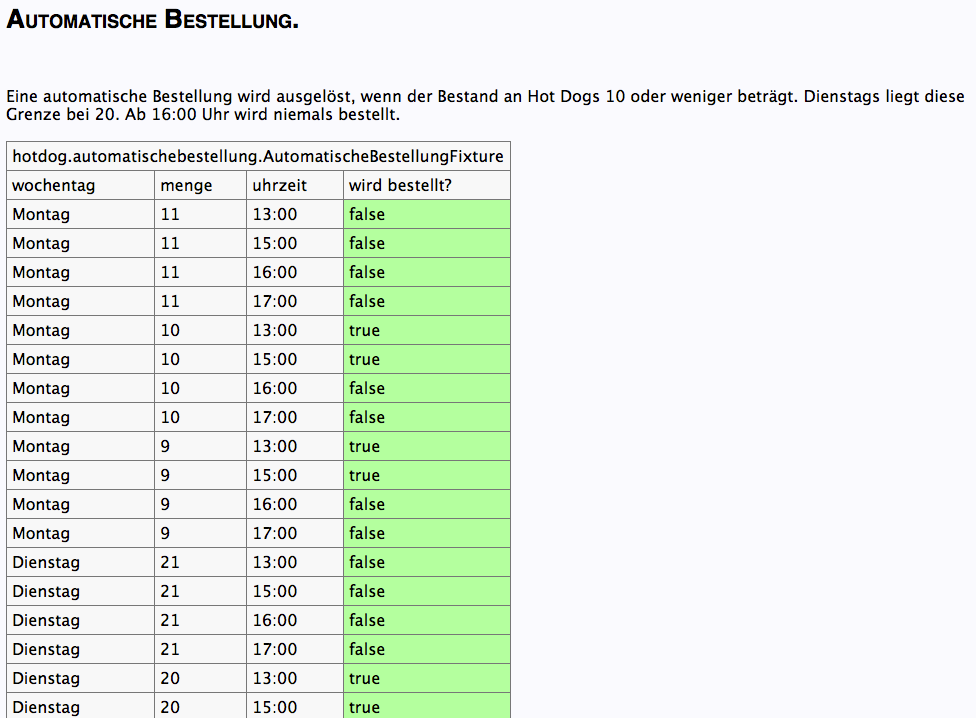
\includegraphics[height=7cm]{SchlechtesBeispiel.png} \newline
\end{center}

\end{frame}

%%%%%%%%%%%%%%%%%%%%%%%%%%%%%%%%%%%%%%%%%%%%%%%%%%
\begin{frame}{Beispiel 2}

\begin{center}
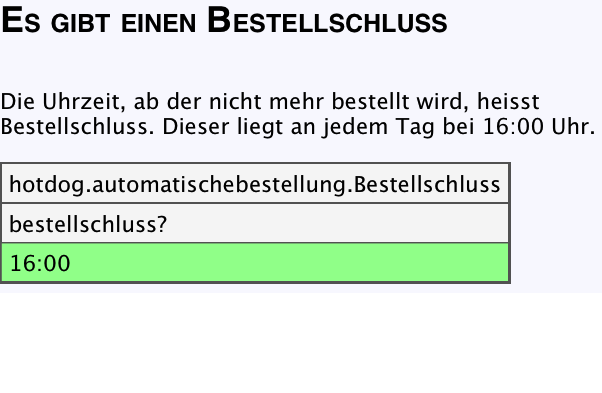
\includegraphics[width=5cm]{bestellschluss.png}
\hfill{}
\onslide+<2->
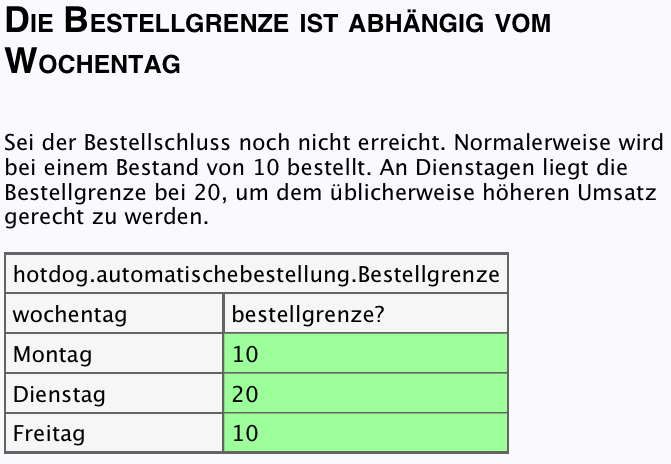
\includegraphics[width=5cm]{wochentag.png}
 \newline
\onslide+<3->
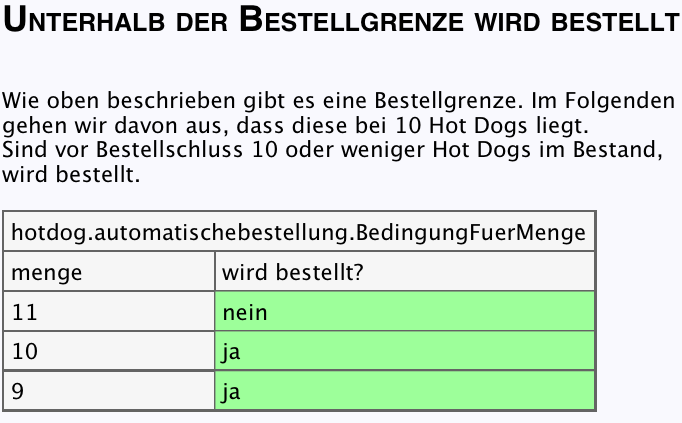
\includegraphics[width=5cm]{bestellgrenze.png}
\hfill{}
\onslide+<4->
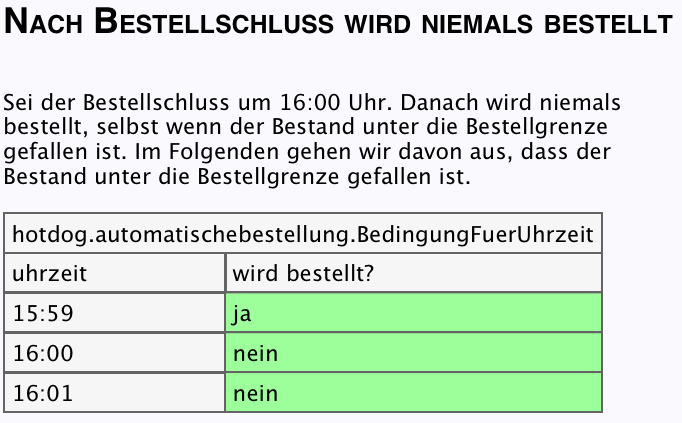
\includegraphics[width=5cm]{keineBestellungNachBestellschluss.png} 
\end{center}

\end{frame}

%%%%%%%%%%%%%%%%%%%%%%%%%%%%%%%%%%%%%%%%%%%%%%%%%%
\begin{frame}{Fazit}

\begin{itemize}
	\item Zentraler Aspekt ist Kommunikation im Specification Workshop
	\item Wesentliche Ergebnisse:
	\begin{itemize}
		\item Eine fachliche Modellierung der Domäne
		\item Ausführbare Spezifikationsbeispiele (Tests)
	\end{itemize}
	\item Spezifikation geht alle an (Auftraggeber, Entwickler, QA, Support)
	\item Dann ist es möglich, eine Quelle für Anforderungen und Dokumentation mit Verbindung zur Anwendung zu haben
\end{itemize}

\end{frame}

%%%%%%%%%%%%%%%%%%%%%%%%%%%%%%%%%%%%%%%%%%%%%%%%%%
\begin{frame}{Bücher zum Thema}

\begin{center}
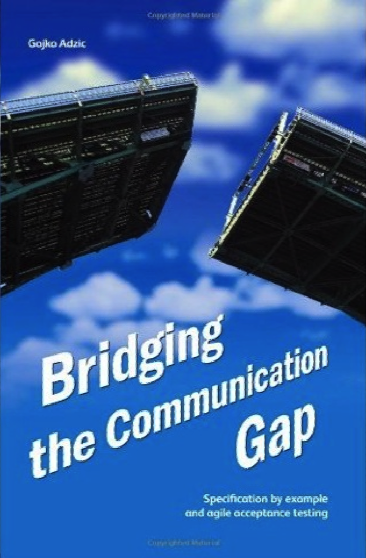
\includegraphics[height=7cm]{CommunicationGap.png}
\hfill

\includegraphics[height=7cm]{SpecificationByExample.png}
\end{center}

\end{frame}

%%%%%%%%%%%%%%%%%%%%%%%%%%%%%%%%%%%%%%%%%%%%%%%%%%
{
\usebackgroundtemplate{
\includegraphics[width=\paperwidth,height=\paperheight]{background-slide.png}}
\begin{frame}{Vielen Dank!}

        Folien auf GitHub:
        \vspace{-0.8em}
        \begin{center}
                \url{https://github.com/leider/Beispielhaft}
        \end{center}

        \begin{block}{Andreas Leidig}
        \begin{description}[Twitterxx]
                \item[E-Mail]  \href{mailto:andreas.leidig@msg-gillardon.de}{\texttt{andreas.leidig@msg-gillardon.de}}
                \item[Twitter] \href{http://twitter.com/leiderleider}{\texttt{@leiderleider}}
        \end{description}
        \end{block}

        \begin{block}{Nicole Rauch}
        \begin{description}[Twitterxx]
                \item[E-Mail]  \href{mailto:nicole.rauch@msg-gillardon.de}{\texttt{nicole.rauch@msg-gillardon.de}}
                \item[Twitter] \href{http://twitter.com/NicoleRauch}{\texttt{@NicoleRauch}}
        \end{description}
        \end{block}
\end{frame}
}
